\documentclass{ws-jmrr}

\usepackage{graphicx}
\usepackage{amsmath}
\usepackage{amssymb}
\usepackage{cite}
\usepackage{gensymb}
\usepackage{enumitem}
\newcommand{\MATLAB}{{\textsc{Matlab}}}

\newcommand\myfigure[1]{%
\medskip\noindent\begin{minipage}{\columnwidth}
\centering%
#1%
%figure,caption, and label go here
\end{minipage}\medskip}

\begin{document}

\catchline{0}{0}{2013}{}{}

\markboth{Julien Leclerc, Aaron T. Becker, Nikolaos V. Tsekos, K\'evin Berger and Jean L\'ev\^eque}{Design and simulation of a superconducting magnetic system for milli/microrobotics applications}

\title{Design and simulation of a superconducting magnetic system for milli/microrobotics applications}

\author{Julien Leclerc$^{~a}$, Aaron T. Becker$^{~a}$, Nikolaos V. Tsekos$^{~b}$, K\'evin Berger$^{~c}$ and Jean L\'ev\^eque$^{~c}$}

\address{$^a$Dept. of Electrical and Computer Engineering, University of Houston, Houston, TX 70004, USA\\
E-mail: jleclerc@central.uh.edu}

\address{$^b$Dept. of Computer Science, University of Houston, Houston, TX 70004, USA}

\address{$^c$GREEN Laboratory, University of Lorraine, Vandoeuvre-l\`es-Nancy, 54506, France}

\maketitle

\begin{abstract}
Magnetically actuated robots are currently being studied as a potential technology for targeted drug delivery and performing minimally invasive surgery within a human body. 
 Superconducting materials offer the advantages of being able to carry large current densities with low losses compared to regular conductors. Superconduction drastically increases the energy efficiency of the system while reducing its size. It also allows producing a higher magnetic field. This paper presents elements that must be taken into consideration when designing a superconducting system for milli/microrobotics applications. A method to design superconducting Helmholtz coil system is detailed.
\end{abstract}
\begin{multicols}{2}
% no keywords

% For peer review papers, you can put extra information on the cover
% page as needed:
% \ifCLASSOPTIONpeerreview
% \begin{center} \bfseries EDICS Category: 3-BBND \end{center}
% \fi
%
% For peerreview papers, this IEEEtran command inserts a page break and
% creates the second title. It will be ignored for other modes.



\section{Introduction}

Magnetic actuation is a promising technology to control miniature robots. This method removes the need for a complex embedded actuation system. Forces are instead created by external magnets, which makes miniaturization easier. Robots can be as simple as a single magnetic particle \cite{sitti2015biomedical}.\par
Two main applications are foreseen for these magnetic millirobots. Application one is the micro-assembly of microscopic objects where robots are used to move, place, and assemble parts together. The second application is in the medical field where robots could be used to perform highly localized drug delivery or minimally invasive surgery. A controlled magnetic field is produced around a patient to actuate a robot placed inside their body. MRI scanners can be used to produce the required magnetic field. This machine can also be used at the same time to track the position of the robot.\par
The MRI scanner is the most prevalent micro/nano robotic system using superconductors. However, it only uses superconductivity for the constant $B_0$ field. The gradients are generated with resistive coils.  Additionally, the large size and expense of an MRI scanner limits its use in most academic labs.\par
Generating high magnetic fields using electromagnets requires large current densities. With regular conducting materials energy is lost by Joule heating in the resistive conductor.
\begin{figurehere}
\begin{center}
	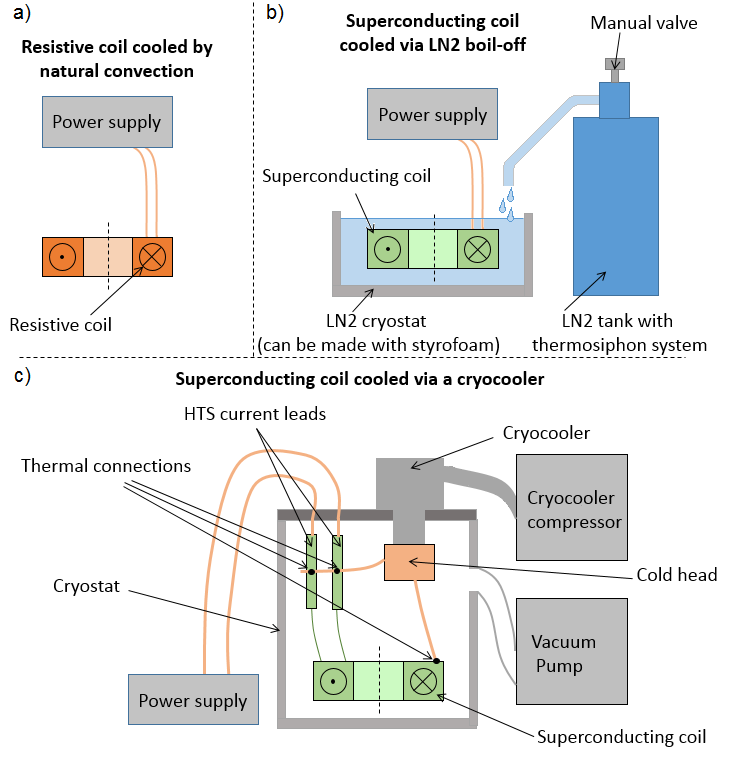
\includegraphics[width=\linewidth]{fig_system_v2.png}
	\caption{Schematic representation of resistive and superconducting magnetic setups with different cooling systems.}
	\label{system}
	\end{center}
\end{figurehere}
\vspace{20mm}
The temperature of resistive coils cannot exceed a certain value that depends on the insulation thermal class. For example, enamel can withstand temperatures up to 105\degree~C.
The maximum current density that can continuously be imposed on a coil depends on the cooling efficiency of the coil. Increasing the current density results in decreasing the size of a solenoid to produce a given magnetic field. Air-cooled solenoids usually can withstand currents densities in the range of 3 to 5 A/mm$^2$. \textbf{Water cooling can drastically increase this value. For example, the 38 T water cooled resistive magnet built at the Nijmegen High Field Magnet Laboratory reaches a current density of 653 A/mm\textsuperscript{2} \cite{mag1 , mag2}. However, resistive electric losses are proportional to the square of the current density. High values of current densities therefore result in large power consumption. The 38 T magnet of the Nijmegen High Field Magnet Laboratory generates 25.5 MW of heat. The amount of water flowing in the magnet to evacuate this energy is equal to 155 l/s.}\par
\textbf{Superconductors are materials that have zero electrical resistivity when cooled below their critical temperature (ranging from 10~K to 108~K for commonly used superconductors). They can transport large current densities with no losses in DC applications. The energy efficiency is therefore drastically improved. Superconduction also enables the coils to be smaller because they can withstand higher current densities. For example, NbTi superconducting wires can carry current densities in excess of 2,500 A/mm$^2$ at 4.2 K and 5 T \cite{muzzi2011test , godeke2007limits}.} The maximum current density a superconductor can carry is limited by a property called the \emph{critical current density} ($J_c$). This value must not be exceeded or the superconductor will heat up and enter the normal (resistive) state which will further increase the temperature and potential lead to damages in the winding.\par
When a superconducting wire is subjected to a varying magnetic field and/or current, an electric field is created inside the material. This electric field together with the current density is a source of losses (called AC losses). These losses must be calculated by engineers to select a cooling device powerful enough to keep the superconductors at the appropriate working temperature. In addition, the heat exchanger must be efficient enough to keep a small temperature difference between the cooling medium and the superconducting wire. A comparison of the physical layout of different cooling systems is presented in fig. \ref{system}.\par
Superconducting magnetic systems offer the following advantages:
\begin{itemize}[leftmargin=*]
\item The size of the windings as well as power supplies are reduced.
\item The energy efficiency is drastically improved.
\item Higher fields can be obtained when other technologies are limited by the heating of the coils.
\item Can create stronger fields than permanent magnets which are limited to a few hundred millitesla.
\end{itemize}
They have some drawbacks:
\begin{itemize}[leftmargin=*]
\item Must be cooled to cryogenic temperatures.
\item The electric current cannot exceed a critical value (temporary overcharge is not possible).
\end{itemize}
Fast moving robotic applications require fast changing magnetic fields. An accurate evaluation of the AC losses is paramount to optimally select the cooling system.\par
\textbf{
This paper proposes using superconductors to control magnetic millirobots. It reviews key elements to consider when designing a superconducting device for this particular application. A method to design superconducting Helmholtz coil systems is presented. This method was programed in \MATLAB ~software and a graphical user interface was made. The computation is fully automated. The source code is attached to this paper and can be used as a tool to perform fast preliminary designs of superconducting magnetic systems.}\par

\emph{Helmholtz coil} systems are composed of two circular electromagnets oriented along the same axis. They are usually used to produce approximately uniform magnetic fields. To ensure proper field uniformity, the radius of the coils should be equal to the distance separating them. In this paper, the term Helmholtz coil is used to describe the more general case where the coils can be separated by a distance different from their radius. If these values are far from each other, the magnetic field inhomogeneity increases. However, having this additional degree of freedom increases the design flexibility. Magnetic robots do not necessary need a homogeneous field. Their small size allows assuming a constant applied flux density throughout the robot. In addition, the controller can be used to compensate for changes in magnetic field when the robot moves by modifying the current supplied to the electromagnets.

\section{Electromagnetic properties of Superconductors}
\label{elec}
Superconductors are characterized by their critical temperature $T_c$. When they are cooled below $T_c$, their electrical resistivity abruptly vanishes. They are, however, not perfect conductors. A phenomenon called flux creep \cite{feigel1989theory} produces a small electric field inside the conductor. The electric field value depends on the current density value, the temperature, and the magnetic field. It has a highly non-linear behavior. It is usually modeled via the well-known power law \cite{ONOGI1989991} presented in eq. 1.
\begin{align}
\frac{\vec{E}}{E_c}&=\left (\frac{|\vec{J}|}{J_c(\vec{B})}  \right )^{n(\vec{B})}\cdot \frac{\vec{J}}{|\vec{J}|}
\label{powerlaw}
\end{align}
In this equation $J_ c$ is the critical current density. It is defined as the current density necessary to produce an electrical field inside the superconductor equal to a value called the critical electric field $E_c$. The value for $E_c$ is normative. It is equal to 0.1 $\mu$V/cm for Low Temperature Superconductors (LTS, $T_c<30K$) and 1 $\mu$V/cm for High Temperature Superconductors (HTS, $T_c \geq 30K$). $n$ is simply called the exponent of the power law, and is a function of the field and temperature.\par
When designing a superconducting coil, the current density $J$ present in the superconductor must stay under the critical value $J_c$. $J_c$ varies both with the temperature and the magnetic field. An increase in temperature or an increase of magnetic field produces a decrease of $J_c$. For most applications, the temperature can be assumed to be constant. The following equation presents a model for the field dependance of $J_c$ of an isotropic superconductor: 

\begin{align}
J_c(\vec{B})&=\frac{J_{\textrm{c0}}}{1+\frac{|\vec{B}|}{B_0}}
\label{model1}
\end{align}

Superconducting wires usually have isotropic behavior, however, superconducting tapes have anisotropic electromagnetic properties and in this case the following model can be used:
\begin{align}
J_c(\vec{B})&=J_c(\vec{B_{\perp}}+\vec{B_{\parallel}})=\frac{J_{\textrm{c0}}}{1+\frac{\sqrt{|\vec{B_{\parallel}}|^2+k^2|\vec{B_{\perp}}|^2}}{B_0}}
\label{model2}
\end{align}
where $\vec{B_{\perp}}$ and $\vec{B_{\parallel}}$ are the components of the magnetic flux density perpendicular and parallel to the superconducting tape respectively.\par
The magnetic field present on the superconductor is the sum of the external magnetic field and the self-magnetic field (magnetic field produced by the superconductor on itself). In some applications the first term may be zero. However, the self-magnetic field is always present and must be taken into account. \par
Some superconducting materials exhibit \emph{anisotropic behaviors} where the reduction of the critical current density depends on the orientation of the magnetic field. In that case, the angle of the magnetic field must be taken into account during the calculations.\par
The critical current density of superconducting tapes or wires is also affected by the mechanical stress it must withstand. Superconductor manufacturers provide the value of the critical tensile strength. For example, the Sumitomo BiSCCO type H tape has a critical tensile strength of 130 MPa. This value corresponds to the tensile strength that produces a decrease of 5\% of the critical current density. This value should not be exceeded.\par
Superconductors are also sensitive to the bending radius. Each manufacturer provides a minimum bending radius. For example, the YBCO tape from Superpower Inc. can be bent to a radius of 5.5 mm.


\section{AC losses}
\label{ac}
A time-varying magnetic field present on the superconductor produces an electric field which, together with the current density produces AC losses. To properly select the cryogenic cooling system, the amount of AC losses must be calculated. However, the highly non-linear behavior of superconductors makes the task difficult. Three options are currently available to calculate AC losses.\par
The first method is based on analytical calculations \cite{0022-3727-3-4-308}. Models are derived from the critical state assumption which assume an infinite value for $n$. This leads to a calculation errors that are large for low $n$ values but decreases to zero when the value of $n$ tends to infinity. The main advantage of this method is that predictions are fast to compute.\par
The second method is based on finite elements calculation \cite{brambilla2006development}. The local variables $E$ and $J$ must be calculated at each point of the superconductor as a function of the time. The amount of losses produced per period is obtained by integrating $E\cdot J$ over the total volume of superconductor and over a period of the input signal. This method is accurate but slow.\par
The last possibility is to use empirical models based on FEM simulations. These models are built by fitting large amounts of data generated via FEM computation. In \cite{leclerc2016artificial} an artificial neural network was trained to fit losses data calculated for a superconducting filament submitted to a rotating, pulsating, or elliptical magnetic field. This type of model requires a long build time because many numerical simulations must be computed. However, once the parameters of the model are found, the predictions are fast and accurate.

\section{Cryogenic cooling system}

Cooling methods for superconducting devices can be classified into two categories: cooling via a cryogenic liquid and cooling via a cryocooler. Figure \ref{system} is a schematic representation of two cooling methods for superconductors and a comparison with a natural convection-cooled resistive coil.\par
Cryogenic fluids commonly used in superconductivity are liquid Helium (LHe, 4.2 K) and liquid Nitrogen (LN2, 77 K). Cryogenic liquids are usually used at their boiling temperature. This ensures that the system is working at a constant temperature. The heat is removed via the evaporation of the liquid. LHe, for example, has a latent heat of vaporization equal to 20.9 J/g at 4.2 K. That means that 1 g of LHe will evaporate to extract 20.9 J of heat. With this value and knowing the quantity of losses produced, the amount of liquid evaporated per unit time can be calculated. LHe is expensive (currently around 6 USD/l) and evaporated gas must be stored to be reliquified. On the other hand, LN2 is cheap (currently around 0.50 USD/l) and easy to handle.\par
Cryocoolers are machines that use a thermodynamic cycle to generate low temperature. They have the advantage of being closed systems (no gas or liquid is lost). Unlike cooling with a cryogenic liquid, this system does not need regular refills. It only needs an electrical power supply to work. The coefficient of performance (COP) of cryocoolers is an important parameter. It is the ratio of the amount of heat extracted at cryogenic temperature and the amount of mechanical work needed. This characterizes the efficiency of the cooling system. The COP decreases when the working temperature decreases. For example, the AL125 refrigerator from Cryomech uses 3,900 W of electric power to extract 100 W of heat at 65K while the AL325, which is designed to work at lower temperature, uses 11,200 Wof electric power to extract the same heat at 25 K \cite{WinNT}. For systems producing a significant amount of AC losses, it is usually chosen to work with HTS rather than LTS to reduce the power consumption of the cooling system.\par
There are three ways to thermally connect a superconducting coil to a cryocooler:
\begin{itemize}[leftmargin=*]
\item Thermal connection via conduction: the coil and the cold head of the cryocooler are placed under vacuum. A highly thermally conductive part connects the coil to the cold head. This part is often a copper braid with a large section.
\item Thermal connection via convection: A cryogenic gas (usually Helium gas) circulates between the superconducting coil and the cryocooler cold head. A heat exchanger is present in both sides. A cryogenic fan is usually used to force the convection.
\item  Thermal connection via boil off of cryogenic liquid: The superconducting coil is placed into a cryogenic liquid bath. The energy dissipated into the coil produces the evaporation of liquid. The cryocooler is used to re-condensate the evaporated liquid. This method is used in zero boil-off MRI scanners.
\end{itemize}

\section{Design of a Superconducting Helmholtz coil system}
\subsection{Magnetic field computation}
As stated in section \ref{elec}, the critical current density of superconductors varies with the magnetic field. One therefore have to calculate its value. The system is axisymmetric. It was chosen to perform the calculations in a 2d axisymmetric coordinate system (see Fig. \ref{coils}). The total magnetic field is the sum of the external and self-magnetic field (see Section \ref{elec}). The external magnetic field depends on the environment. The self-magnetic field is produced by the coil itself and must be computed.\par
Each coil has a total number of turns equal to $N$. A current $I_w$ circulates in the conductor. The current density averaged over the superconducting wire cross-section is $J_w=I_w/S_w$ where $S_w$ is the superconducting wire cross section area. The cross-section of the coil is composed of areas occupied by the superconducting wire and area occupied by insulating material. The filling factor of the coil is $C_{\textrm{ff}}=N\cdot S_w/((R_e-R_i)\cdot T)$ where $R_e$ and $R_i$ are the external and internal radius of the coils respectively and $T$ is the their thickness (see Fig. \ref{coils}).\par
To perform the self-magnetic field calculation, the current density is averaged over the coil cross section i.e. the non-uniformity produced by the combination of insulating and conducting material on the current density is neglected.  
\begin{figurehere}
	\begin{center}
	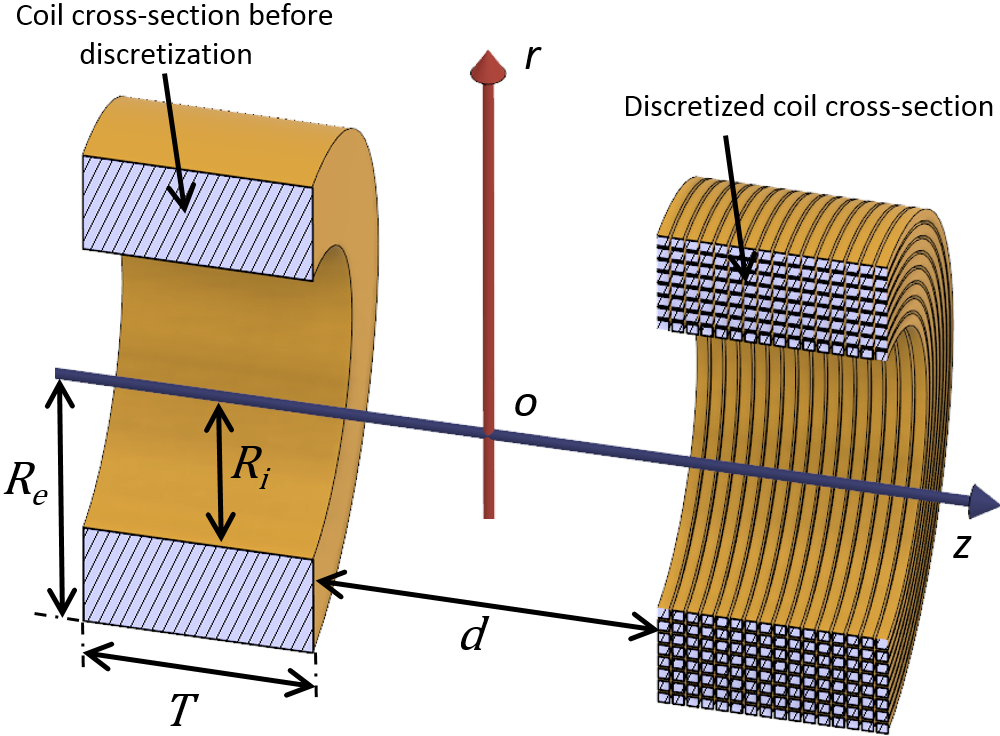
\includegraphics[width=\linewidth]{coil_system.png}
	\caption{Drawing of the Helmholtz coil system.}
	\label{coils}
	\end{center}
\end{figurehere}
The current density averaged over the coil cross section is denoted $J_a$ and is calculated with $J_a=C_{\textrm{ff}}.J_s$.\par 
Each coil can be decomposed into a sum of infinitesimal current loop having a cross section $dr.dz$. The magnetic flux density $dB_z(R_p,Z_p,R_m,Z_m)$ and $dB_r(R_p,Z_p,R_m,Z_m)$ produced by a current loop can be calculated using the semi-analytical equations 3, 4, 5 and 6 \cite{simpson2001simple}. In these equations, the field calculation point is placed at coordinates $(R_m,0,Z_m)$ in the cylindrical coordinate system and the current loop is placed at $z=Z_p$ and has a radius $R_p$. The magnetic flux density produced by the complete coil is obtained by performing the integration of $dB_z(R_p,Z_p,R_m,Z_m)$ and $dB_r(R_p,Z_p,R_m,Z_m)$ over the coil cross section (see eq. 7 and 8).

\begin{align}
\begin{split}
dB_z(R_p,Z_p,R_m,Z_m) =&\frac{\mu _0I}{2\pi\delta ^{2}\beta  }( [ \left ( R_p^2-R_m ^2-(Zm-Zp)^2 \right )\\
&.(E(k^2)+\delta ^2K(k^2)) ) ]
\end{split}
\label{Bz1loop}\\
\begin{split}
dB_r(R_p,Z_p,R_m,Z_m) =&\frac{\mu _0 I \cdot (Zm-Zp)}{2\pi\delta ^{2}\beta R_m   }( [ \left ( R_p^2-R_m ^2-z^2 \right )\\
&.(E(k^2)-\delta ^2K(k^2))) ]
\end{split}
\end{align}
\begin{align}
%\label{Bteta1loop}\\
&\delta =\sqrt{R_p^2+R_m^2+(Z_m-Z_p)^2-2R_pR_m}
\label{delta}\\
&\beta =\sqrt{R_p^2+R_m^2+(Z_m-Zp)^2+2R_pR_m}
\label{beta}\\
&B_z(R_m,Z_m)=\int_{d}^{d+T}\int_{R_i}^{R_e}dB_z((R_p,Z_p,R_m,Z_m))dR_pdZ_p\\
%\label{Bztot}\\
&B_r(R_m,Z_m)=\int_{d}^{d+T}\int_{R_i}^{R_e}dB_r((R_p,Z_p,R_m,Z_m))dR_pdZ_p
%\label{Brtot}\\
\end{align}
\begin{figurehere}
\begin{center}
	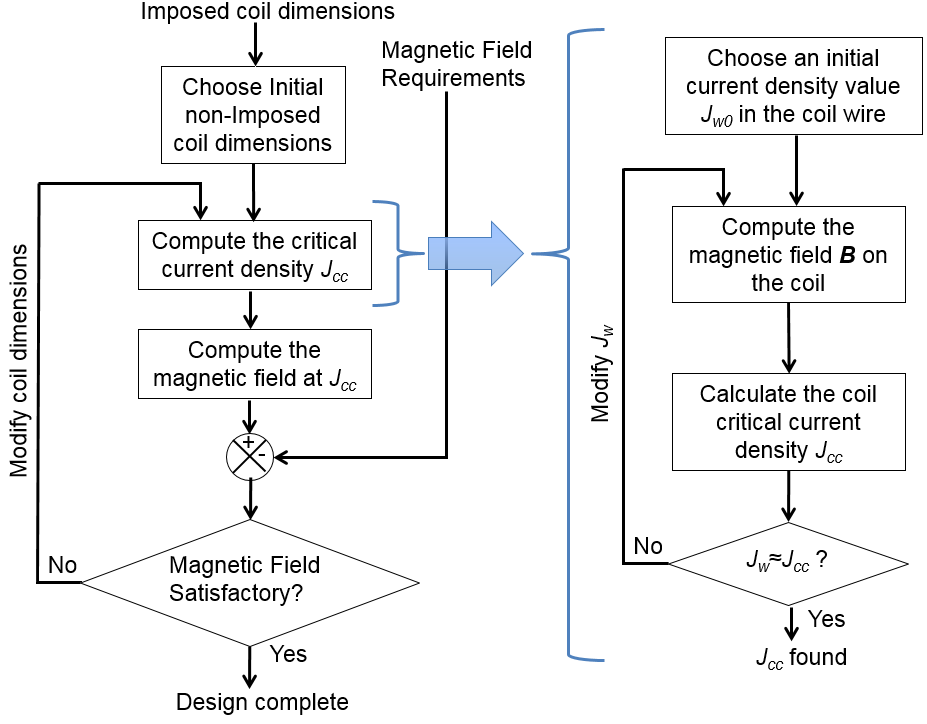
\includegraphics[width=\linewidth]{method.png}
	\caption{Block diagram presenting the method used to compute the coil critical current density $J_{\textrm{cc}}$ (b) and optimize the coils geometry (a).}
	\label{method}
	\end{center}
\end{figurehere}
\subsection{Critical current density computation}
\label{jccalc}
It is first necessary to clarify the difference between the local critical current density $J_c$ and the coil critical current density $J_{\textrm{cc}}$. At each point on the coil, the superconductor is subjected to a different magnetic field $B(R_m,Z_m)$ \cite{linares2016design}. The critical current is a function of the magnetic field as shown in the model presented in eq. \ref{model1}. Therefore, at each location of the coil, a value for $J_c(B)$ can be calculated. It correspond to the maximum current density the superconductor can carry \textbf{at this point}. On the other hand, the value of $J_{\textrm{cc}}$ corresponds to the maximum current density the conductor of \textbf{the complete coil} can carry.\par
In the considered Helmholtz coil problem, the only sources of magnetic field are the coils of the system. There is no external magnetic field. The two coils are connected in series and are therefore sharing the same current. The magnetic field present on the Helmholtz coils system is thus proportional to the current and is classified as self-magnetic field.\par
$J_w$ is constant in the in the winding since it is made with a single conductor. Therefore, much like with the weak chain link problem, the maximum current density $J_{\textrm{cc}}$ that the coil can carry correspond to the minimum $J_c$ value encountered in the winding when $J_w=\textrm{min}(J_c)$. The problem is not straightforward to solve: a change in the value of $J_w$ produces a change in $\textrm{min}(J_c)$ which define the maximum value for $J_w$. An iterative calculation is therefore needed to find $J_{\textrm{cc}}$ (see fig. \ref{method} (b)).\par
The method used to solve this problem is the following: first, a starting value $J_{w0}$ is chosen for $J_{w}$. The magnetic field produced at this current is calculated. From this results, $J_c$ is calculated over the coils cross section. $\textrm{min}(Jc)$ is compared to $J_w$. If $J_w>\textrm{min}(J_c)$ the current density $J_w$ needs to be decreased in the next iteration. If $J_w<\textrm{min}(J_c)$ the current density $J_w$ needs to be increased in the next iteration. The process is repeated until the condition $J_w=\textrm{min}(J_c)$ is satisfied (or close to be satisfied) and therefore $J_{\textrm{cc}}$ is found.\par
This algorithm was implemented in the provided \MATLAB ~function \emph{JcSearch.m}. The optimization algorithm \texttt{fminsearch} was used to search $J_{\textrm{cc}}$.\par
Electromagnetic engineering problems often start with magnetic field requirements and some geometry constraint. Here, the case where a magnetic flux density $B_{\textrm{obj}}$ needs to be generated at the center of the system will be solved. Additional geometric constraints are, imposed values for $R_i$ and $d$ and, a square cross section for the coils i.e. $R_e-R_i=T$. The only parameter that can be adjusted is $T$.\par

\subsection{Coil geometry optimization}
An optimization algorithm is used to find the correct value of $T$ (see fig. \ref{method} (a)). An initial value must first be chosen. In the provided code, the initial value is equal to $R_i$. Then, the developed \MATLAB ~function \emph{JcSearch.m} described in \ref{jccalc} is used to compute $J_{\textrm{cc}}$. The magnetic flux density can then easily be calculated at the center of the system for this current density value. The optimization algorithm compares the obtained field with the objective value. It then modify the value for $T$ and iterates the process until a satisfactory field value is found. The optimization algorithm used is the function \texttt{fminsearch} of \MATLAB. It uses the Nelder-Mead simplex algorithm \cite{lagarias1998convergence} to generate the values for $T$. The cost function it minimizes is presented in eq. \ref{CostFct} where $B(T)$ is the magnitude of the flux density at the system center and at critical current value for a give value for T. The coil geometry optimization was implemented in the provided \MATLAB ~function \emph{TSearch.m}.

\begin{align}
\textrm{CostFct}(T)=\left ( B(T)-B_{\textrm{obj}} \right )^{2}
\label{CostFct}
\end{align}

\subsection{AC Losses computation}
\label{aclosses}
The results from the magnetic field computation and critical current density can be used to evaluate the superconducting magnetization AC loses (see Section \ref{ac}). An analytical model was used to perform this calculation. The model considered is presented in \cite{zhang2003angular} and eq. \ref{Weq} where $2\cdot a$ is the width of the superconducting tape and $y$ is the parameter characterizing the anisotropy of the superconductors. The applied current and magnetic field are sinusoidal. The authors of this model based their calculations on the critical state assumption \cite{bean1962magnetization} and take into account the effect of the magnetic field angle. To test their model they calculated losses for a BiSCCO tape and used a value of 10 for $y$. \par
The unit of the obtained magnetization losses $W$ is J.m\textsuperscript{-3}.cycle\textsuperscript{-1}. It corresponds to the energy dissipated into 1~m\textsuperscript{3} of superconductor during one period of the signal. It is independent of the frequency $f$. The power $P$ (in Watts) dissipated in 1~m\textsuperscript{3} of superconductor can be easily calculated with $P=W\cdot f$. 
\begin{align}
\begin{split}
W=\frac{2\mu_0a^2Jc^2}{3}\left ( \left (\frac{3\left |B  \right |}{\mu_0aJc}-2  \right  )+\left (\frac{\left |B  \right |}{\mu_0aJc}+\frac{2J}{Jc}  \right )\frac{J}{Jc}\right ) \\ \left ( y^2\cos^2(\alpha )+\sin^2(\alpha ) \right )
\label{Weq}
\end{split}
\end{align}
   

\subsection{Practical example}

Assume we want to calculate an Helmholtz coil system that produces a magnetic flux density of 1.5 T in its center and that is large enough to accommodate a person. The internal diameter of the coils is chosen to be equal to 0.7 m. The distance between the coils $d$ is imposed to be 0.4 m. A square cross-section for the coils is also imposed i.e. $R_e-R_i=T$. The only parameter that can be adjusted to obtain the desired flux density is therefore the length of the side of the square cross-section $T$. A security factor will be taken on the maximum current value: the coil will be designed to produce 1.875T at the critical current value. At 1.5 T the current in the coil will be equal to 80\% of the critical value.\par
The material considered in this study is the DI-BiSCCO tape manufactured by Sumitomo Electric Industries. Its critical current density field dependency is modeled by eq. \ref{model2}. At 30K, $J_{c0}$ is approximately equal to 500e6~A/m and $B_0$ is approximately equal to 3 T. These values have been obtained by approximating data provided by Sumitomo Electric Industries. This model takes into account the effect of the magnetic field angle with respect to the tape plane. $B_{\perp}$ is the component of the flux density perpendicular to the tape surface (called a-b plane) and $B_{\parallel}$ is the component parallel to the tape surface (c-axis). The parameter $y$ characterizing the anisotropy of the superconductor is assumed to be equal to 10 as in section \ref{aclosses}.\par
These values were entered into the provided \MATLAB ~graphical interface and the computation of the coil geometry was performed. The result of the calculation is presented in fig. \ref{Results}. In this figure, part a) shows the obtained flux density at maximum current. The flux density has a value of 1.87 T, close to the target. The next plot, b), shows a map of the ratio $J_w/Jc$. The maximum value is 1 which shows that the maximum current density is reached without exceeding it. The last graph, c), shows a map of the losses produced in the winding during each cycle. The losses are larger on the sides of the coils. Indeed, at these locations, the magnetic field has a stronger perpendicular component and, accordingly to the model used (eq. \ref{Weq}), more losses are generated there. The total losses obtained are equal to 16,427 J.cycle$^{-1}$ and the value for T is 0.17 m.
\section{Conclusion}
Superconductors could be used advantageously to control magnetically actuated robots because of their high current density capabilities and low losses. They could enable drastically reducing the size of the system while improving its energy efficiency. Superconductors must be cooled at cryogenics temperature. Using cryogenic liquids such as liquid nitrogen (77K) or liquid helium (4.2K) is a possible solution. Cryocoolers can also be used to cool superconductors via conduction heat transfer or reliquefaction of the cryogenic fluid.\par 
\begin{figurehere}
	\begin{center}
	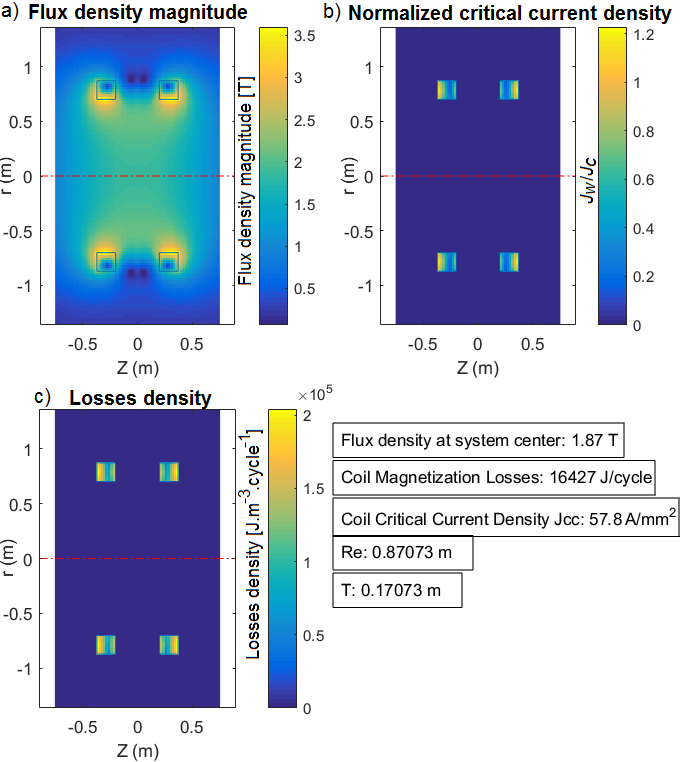
\includegraphics[width=\linewidth]{SimResults.png}
	\label{Results}
	\vspace{-0.5cm}
	\caption{Results from geometric optimization of a superconducting Helmhotz coil system.}
	\end{center}
\end{figurehere}
\vspace{-0.5cm}


A method to design superconducting magnetic systems for microrobotics applications was presented. The design method uses an iterative algorithm to find the critical current of superconducting coils. The self-magnetic field is computed and its effect is taken into account. An optimization method able to find the geometry of a Helmholtz coil system to produce a user defined magnetic field was programed. The \MATLAB ~code and a graphical interface is attached to this paper and available for download.\par
Robotics applications often require fast changing magnetic fields. Under these conditions, AC losses are generated inside the superconductors. These losses must be carefully evaluated to ensure the proper sizing of the cryogenic cooling equipment.\par
The \MATLAB ~program was tested to design an Helmholtz coil system able to generate 1.5T at its center. The optimum geometry was obtained and data about AC losses were computed.\par
Future work should include experimental measurements of AC losses in a superconducting magnetic system. A high-fidelity model for AC losses computation based on finite elements should also be implemented.

\bibliographystyle{unsrt}
\bibliography{biblio}


\end{multicols} 
\end{document}
